\chapter{Implementazione}

Il modello è stato implementato in \texttt{Python} utilizzando la libreria \texttt{scikit-fuzzy}.  
L'intero codice sorgente è disponibile su \href{https://github.com/Leso246/FuzzyACC}{GitHub}.
\\\\
\noindent L'output del sistema fuzzy non è stato utilizzato direttamente, ma sottoposto a un \emph{filtro passa-basso} 
al fine di ridurre la variabilità rapida del segnale ed aumentare il comfort percepito dal conducente.  
Il filtro è descritto dalla seguente equazione:

\[
a_{f}(t) = \alpha \cdot a(t) + (1 - \alpha) \cdot a_{f}(t-1),
\]

\noindent dove:
\begin{itemize}
    \item $a_{f}(t)$ rappresenta l'accelerazione filtrata
    \item $\alpha = 0.1$ è il coefficiente di smoothing scelto
    \item $a(t)$ rappresenta l'accelerazione fuzzy grezza in output
    \item $a_{f}(t-1)$ è rappresenta l'accelerazione filtrata al passo precedente
\end{itemize}
Una visualizzazione interattiva del funzionamento di tale filtro è disponibile 
su \href{https://www.geogebra.org/m/tb88mqrm}{GeoGebra} \cite{geogebraEWMA}.
\\\\
\noindent Inoltre, per eliminare oscillazioni di bassa entità, tutte le accelerazioni con valore assoluto inferiore a $0.12 \, \mathrm{m/s^2}$ 
sono state poste pari a zero.  
Questa soglia consente di evitare micro-variazioni potenzialmente fastidiose. Si noti che un valore troppo elevato potrebbe
generare accelerazioni più brusche nel momento in cui il sistema reagisce a una variazione.
\\\\
\noindent Sia la soglia di $0.12 \, \mathrm{m/s^2}$ sia il coefficiente $\alpha = 0.1$ sono stati scelti empiricamente tramite test, 
bilanciando la reattività del sistema con la stabilità e il comfort del conducente.

\section{Dataset di riferimento e calcoli preliminari}
Per valutare la bontà del modello, è stato utilizzato un dataset pubblico del 2019 \cite{wang2019acc_dataset}, che d'ora in avanti
verrà denominato \texttt{dataset\_reale}, contenente dati raccolti da un veicolo dotato di ACC su un tratto dell'Interstate-65 
(un'autostrada statunitense) per una durata di 15 minuti.  
I dati sono stati acquisiti direttamente tramite l'unità radar di serie del veicolo e il CAN bus.  
I confronti tra dati reali e simulati sono riportati nel Capitolo \ref{cha:risultati}.
\\\\
\noindent Il dataset include le seguenti colonne:
\begin{itemize}
    \item \textbf{timestamps} [s]: istanti di campionamento (frequenza di $10\,\mathrm{Hz}$)
    \item \textbf{ego\_velocity} [m/s]: velocità del veicolo \emph{ego}
    \item \textbf{leader\_velocity} [m/s]: velocità del veicolo \emph{leader}
    \item \textbf{space\_gap} [m]: distanza tra i veicoli
    \item \textbf{ACC command acceleration} [m/s\textsuperscript{2}]: accelerazione richiesta dal sistema ACC per il veicolo \emph{ego}
\end{itemize}

\noindent Per consentire un confronto tra modello e dati reali, nella simulazione sono state calcolate le stesse grandezze riportate di
seguito, aggiungendo le accelerazioni \texttt{ego\_acceleration} e \texttt{leader\_acceleration}.

\subsection{Timestamps}
La simulazione utilizza la stessa frequenza del \texttt{dataset\_reale}, 
ovvero $10\,\mathrm{Hz}$ (0.1 secondi per passo), per un totale di 9000 misurazioni (15 minuti).

\subsection{Ego Acceleration}
L'accelerazione del veicolo \emph{ego} viene calcolata come output del modello fuzzy e filtrata attraverso il filtro EWMA.  
Al tempo $t=0$ l'accelerazione iniziale è impostata a zero.

\subsection{Leader Acceleration}
L'accelerazione del veicolo \emph{leader} viene calcolata a partire dal \texttt{dataset\_reale} come 
variazione di velocità tra due campioni consecutivi:
\[
a_t(\mathrm{leader}) = \frac{v_t(\mathrm{leader}) - v_{t-1}(\mathrm{leader})}{\Delta t}
\]

\subsection{Ego Velocity}
La velocità del veicolo \emph{ego} viene aggiornata ad ogni istante della simulazione.
Come valore iniziale è stato preso il primo campione presente nel \texttt{dataset\_reale}.  
\\\\
\noindent Ad ogni step temporale $\Delta t = 0.1\,\mathrm{s}$, la nuova velocità è calcolata secondo la legge del moto uniformemente 
accelerato:
\[
v_t(\mathrm{ego}) = v_{t-1}(\mathrm{ego}) + a_t(\mathrm{ego}) \cdot \Delta t
\]
dove $a_t(\mathrm{ego})$ è l'accelerazione filtrata in output dal modello del veicolo \emph{ego} al tempo $t$.

\paragraph{Annotazione} Come verrà visto successivamente \textcolor{red}{AGGIUNGI RIFERIMENTO}, l'accelerazione impartita dal modello 
non corrisponderà all'accelerazione effettiva del veicolo nella realtà. Tuttavia, non essendo possibile testare il modello su un veicolo 
reale, questa semplificazione è considerata accettabile per valutare la performance del sistema.

\subsection{Leader Velocity}
La velocità del veicolo \emph{leader} viene copiata direttamente dalla colonna corrispondente del \texttt{dataset\_reale}.

\subsection{Space Gap}
Il valore iniziale dello \texttt{space\_gap} è preso dal primo campione del \texttt{dataset\_reale}.
\\\\
\noindent Ad ogni passo temporale, lo spazio tra i veicoli viene aggiornato come:
\[
\mathrm{space\_gap}_t = \mathrm{space\_gap}_{t-1} + \left( \mathrm{leader\_travelled\_space}_t - \mathrm{ego\_travelled\_space}_t \right)
\]
dove le distanze percorse dai veicoli durante lo step $\Delta t$ sono:
\[
\mathrm{ego\_travelled\_space}_t = v_{t-1}(\mathrm{ego}) \cdot \Delta t + \frac{1}{2} a_t(\mathrm{ego}) \cdot (\Delta t)^2
\]
\[
\mathrm{leader\_travelled\_space}_t = v_{t-1}(\mathrm{leader}) \cdot \Delta t + \frac{1}{2} a_t(\mathrm{leader}) \cdot (\Delta t)^2
\]

\vspace{10mm}
\noindent Per ciascun timestamp vengono inoltre ricalcolati i parametri necessari al modello fuzzy:  
\[
\mathrm{time\_headway}_t = \frac{\mathrm{space\_gap}_t}{v_t(\mathrm{ego})}
\]

\[
\mathrm{relative\_velocity}_t = v_t(\mathrm{leader}) - v_t(\mathrm{ego})
\]

\noindent Questi valori vengono utilizzati come input dal modello per calcolare la nuova accelerazione in output.



% \subsection{Ego Acceleration}
% Nel dataset originale è presente l'accelerazione richiesta dall'ACC, ma questa differisce dall'accelerazione reale del veicolo \emph{leader}.  
% Per questo motivo, l'accelerazione effettiva è stata calcolata come variazione di velocità tra due campioni consecutivi:
% \[
% a_{\mathrm{leader}} = \frac{v_t - v_{t-1}}{\Delta t}
% \]

% \noindent Come evidenziato in Figura \ref{Fig:acceleration_effettiva_impartita}, si conferma che l'accelerazione effettiva 
% del veicolo \emph{leader} differisce da quella impartita dal sistema ACC, principalmente a causa di ritardi meccanici, 
% inerzia del veicolo e condizioni reali della strada.

% \begin{figure}[H]
%     \centering
%     \adjustbox{center}{
%         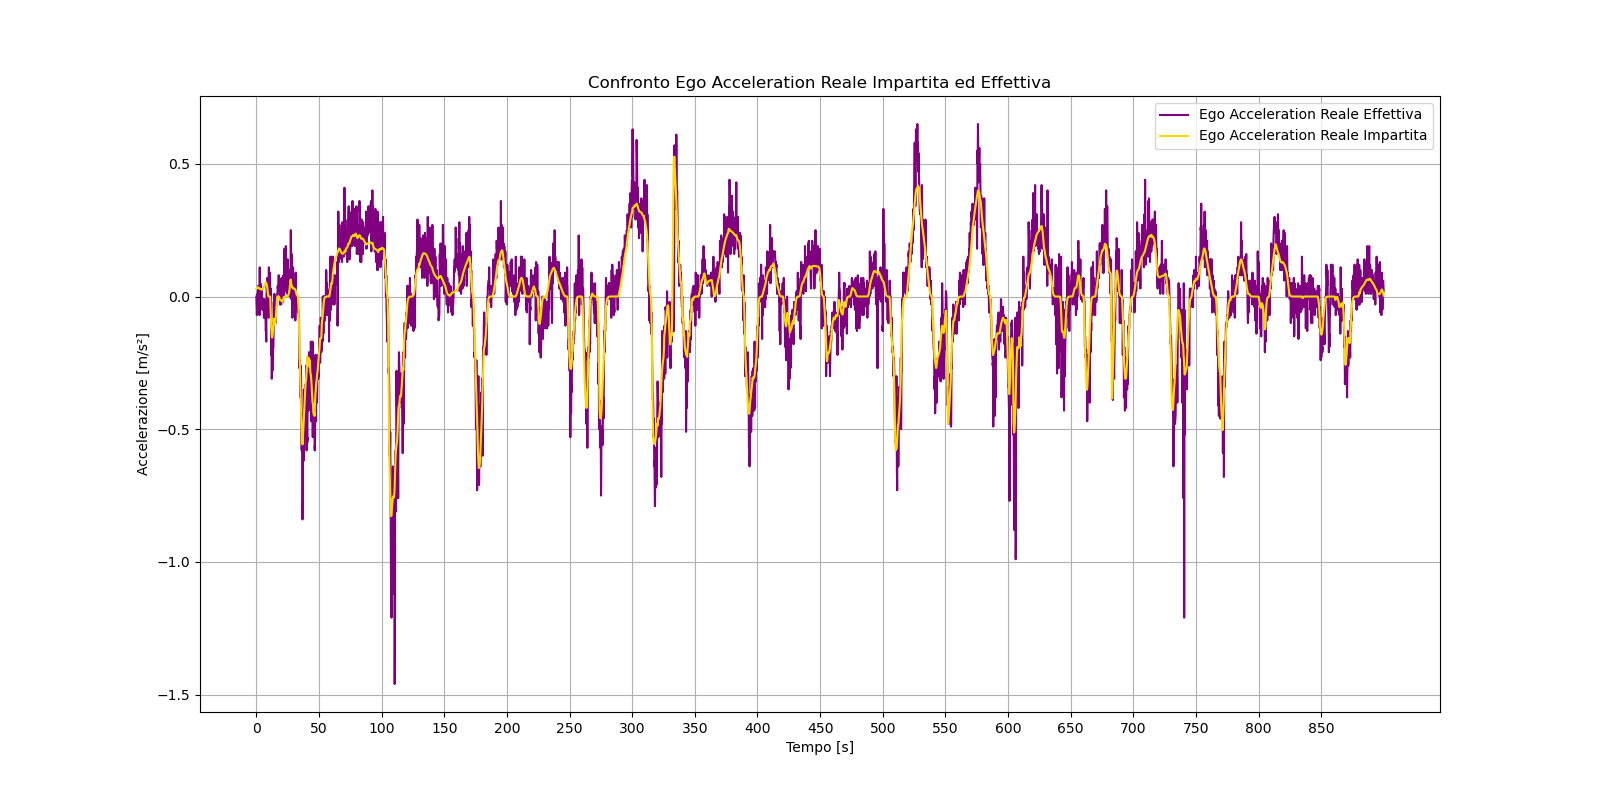
\includegraphics[width=1.5\linewidth]{simulation/real_data_comparison/acceleration_effettiva_impartita.png}
%     }
%     \caption{Confronto tra accelerazione effettiva del veicolo \emph{ego} e accelerazione impartita dal sistema ACC.}
%     \label{Fig:acceleration_effettiva_impartita}
% \end{figure}




